\newif\ifglobal

%%%%%%%%%%%%%%%%%%%%%%%
%%% Compile to view %%%
%%%%%%%%%%%%%%%%%%%%%%%

%%%%%%%%%%%%%%%%%%%%%%%%%%%%%%%%%%%%%%%%%%%%%%%%%%%
%%% Readme:                                     %%%
%%% https://www.overleaf.com/read/bwdjvfjksvjy/ %%%
%%%%%%%%%%%%%%%%%%%%%%%%%%%%%%%%%%%%%%%%%%%%%%%%%%%

% >>> M?: marks a module setting number or important notice

% >>> M4: Set {./relative-path} to external files for this module <<<
\def \modulefiles {./34-WCTRL}
% To add an external file, use:
% (Replace '---' with actual filename)
% '\input{\modulefiles/tables/---.tex}' for tables
% '\includegraphics{\modulefiles/figures/---}' for figures
% '\subfile{\modulefiles/---}' for register files


% >>> M1: This module is in global project? <<<
% 'YES' - uncomment; 'NO' - comment out
\globaltrue

\ifglobal
    \documentclass[main\_\_CN.tex]{subfiles}

\else
    % Font "FandolSong-Regular" used by ctex does not have GSUB table.
    % It causes warnings that do not affect compilation and can be ignored.
    \PassOptionsToPackage{quiet}{fontspec}

    \documentclass[openany, 10pt]{book}

    % >>> M2: In ./00-shared/preamble-trm-module, also find
    %         settings for visibility of todo notes, watermark <<<
    \usepackage{preamble-trm-module}


    % Enable Chinese typesetting
    \usepackage{ctex}

    % >>> M3: Temporary labels in Chinese
    %         you can add your own labels there <<<
    \myexternaldocument{./00-shared/temp-labels-cn}

\fi %\ifglobal


\setcounter{secnumdepth}{4}


% >>> M5: If this module needs any updates in
% './00-shared/preamble-trm-module.sty'
% (include additional package, etc.), contact your module PM
% or create the file './00-shared/changelog.tex' make the
% necessary updates yourself and document them in this file <<<


\begin{document}


% Sets language into which pre-defined bits of text are translated
\selectlanguage{chinese}

% Do not delete this block
\ifglobal
% Add the following front matter if
% this module is outside of global project
\else
    \InputIfFileExists{readme}{}{}
    {\let\clearpage\relax \listoftodos}
    {\let\clearpage\relax \listofdonetodos}
    \tableofcontents
    %\listoftables
    %\listoffigures
\fi


\hypertarget{wctrl}{}
\chapter{World 控制器 (WCL)}\label{mod:wctrl}

\section{概述}

\chipname{} 允许用户将芯片的硬件和软件资源分为安全世界 (World0) 和非安全世界 (World1)，从而有效防止非法数据拷贝、破坏或篡改，或通过恶意软件、硬件监视、硬件干预等方式破坏或获取设备信息。两个世界之间可以由 World 控制器进行切换。

默认情况，\chipname{} 不划分安全世界和非安全世界，所有资源全部共享。如有需求，用户可通过权限配置将资源分为安全世界和非安全世界，具体配置请见章节 \ref{mod:permctrl} \textit{\nameref{mod:permctrl}}，本章节仅介绍 World 控制器及 CPU 在两个世界之间的切换。

\section{主要特性}
\label{sec:alias-features}

\chipname{} 的 World 控制器主要用于：
\begin{itemize}
    \item 控制 CPU 在安全世界与非安全世界中的相互切换
    \item 记录 CPU 的世界切换信息
\end{itemize}

\section{功能描述}
\label{sec:34-WCTRL-func-descr}

在 World 控制器的帮助下，\chipname{} 的安全世界和非安全世界可访问的资源可以不同：

\begin{itemize}
    \item 安全世界 (World0)：
    \begin{itemize}
        \item 可以访问所有的外设和存储空间。
        \item 主要执行所有需要保密的操作，如用户认证、安全通信和数据加解密等。
    \end{itemize}
    \item 非安全世界 (World1)：
    \begin{itemize}
        \item 只能访问部分的外设和存储空间。
        \item 执行其他操作，如用户操作系统、各种应用程序等。
    \end{itemize}
\end{itemize}


\chipname{} 的 CPU 和从设备均有相应的安全世界和非安全世界权限：
\begin{itemize}
    \item CPU 可以在两个世界中运行：
        \begin{itemize}
            \item 在安全世界：运行安全世界的程序
            \item 在非安全世界：运行非安全世界的程序
            \item CPU 上电时均默认处于安全世界，此后可通过配置 World 控制器在两个世界间进行切换。
        \end{itemize}
    \item 所有的从设备（外设\hyperref[note:wctrl-access]{*}、存储器等）均可分别配置：
        \begin{itemize}
            \item 安全世界权限：表示可以从安全世界访问，即允许 CPU 从安全世界中访问该从设备；
            \item 非安全世界权限：表示可以从非安全世界访问，即允许 CPU 从非安全世界中访问该从设备。
            \item 注意，从设备可配置为同时具有安全世界和非安全世界权限。
        \end{itemize}
        具体请见章节 \ref{mod:permctrl} \textit{\nameref{mod:permctrl}}。
\end{itemize}

\begin{tiplisting}\label{note:wctrl-access}
World 控制器本身也属于一种外设。因此，与所有从设备一样，World 控制器理论上也可以配备安全世界和非安全世界的访问权限，即允许从安全世界和非安全世界访问 World 控制器。不过，为了保证世界切换的安全性，应\textbf{禁止} World 控制器的非安全世界访问权限，确保 CPU 无法从非安全世界中更改 World 控制器的配置。
\end{tiplisting}

\textbf{CPU 在访问从设备时：}

\begin{enumerate}
    \item 首先，CPU 将告知从设备自己所处的世界；
    \item 接着，从设备会根据自身的权限配置，判断是否允许 CPU 的访问。
        \begin{itemize}
        \item 如果允许访问，则访问继续；
        \item 如果不允许访问，则不响应此次访问并且触发中断。
        \end{itemize}
\end{enumerate}
这样一来，可以保证安全世界的资源不会被非安全世界非法访问。

注意，下述 CPU 中断相关的 CSR 寄存器只能在安全世界执行写操作，在非安全世界只能读不能写，从而确保中断只能由安全世界控制。
\begin{table}[H]
    \centering
    \begin{tabular}[c]{ | l | l | l | l | }
    \hline\rowcolor{lightgray}
    \textbf{名称} & \textbf{描述} & \textbf{地址} & \textbf{访问} \\ \hline
    \multicolumn{4}{|l|}{\textbf{机器模式异常设置 CSR}} \\\hline
    \hyperref[regdesc:MSTATUS]{mstatus} & 机器模式状态寄存器 & 0x300 & 读/写 \\\hline
    \hyperref[regdesc:MTVEC]{mtvec}  & 机器模式异常向量寄存器 & 0x305 & 读/写 \\\hline
    \multicolumn{4}{|l|}{\textbf{机器模式异常处理 CSR}} \\\hline
    \hyperref[regdesc:MSCRATCH]{mscratch} & 机器模式暂存寄存器 & 0x340 & 读/写 \\\hline
    \hyperref[regdesc:MEPC]{mepc} & 机器模式异常程序计数器 & 0x341 & 读/写 \\\hline
    \hyperref[regdesc:MCAUSE]{mcause}  & 机器模式异常原因寄存器 & 0x342 & 读/写 \\\hline
    \hyperref[regdesc:MTVAL]{mtval} & 机器模式异常值寄存器 & 0x343 & 读/写 \\\hline
    \end{tabular}
\end{table}


\section{CPU 的世界切换} \label{sec:34-WCTRL-recommended-operation}

CPU 可以从安全世界切换至非安全世界，也可以从非安全世界切换至安全世界。

\subsection{安全世界切换到非安全世界}\label{sec:34-WCTRL-safe-nosafe-switch}

\begin{figure}[H]
    \centering
    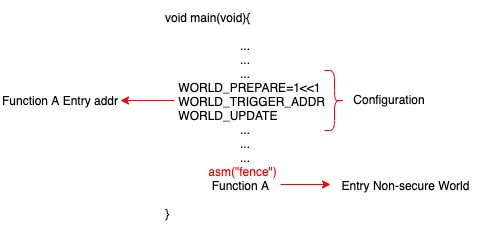
\includegraphics[width=0.7\textwidth]{./34-WCTRL/figures/world0toworld1.png}
    \caption{安全世界切换到非安全世界}
    \label{fig:34-WCTRL-safe-nosafe-switch}
\end{figure}
当\chipname{} 的 CPU 准备从安全世界切换至非安全世界并执行非安全世界程序时，只需完成如下步骤：






\begin{enumerate}
    \item 配置 \hyperref[regdesc:WCLCORE0WORLDPREPAREREG]{WCL\_CORE\_0\_WORLD\_PERPARE\_REG} 寄存器为 0x2，表示要切换至进入非安全世界。
    \item 配置 \hyperref[regdesc:WCLCORE0WORLDTRIGGERADDRREG]{WCL\_CORE\_0\_World\_TRIGGER\_ADDR\_REG} 寄存器为非安全世界的入口地址，即需要执行的非安全世界应用程序的入口地址。
    \item 配置 \hyperref[regdesc:WCLCORE0WORLDUPDATEREG]{WCL\_CORE\_0\_World\_UPDATE\_REG} 寄存器（可配置任意值），代表已完成配置。
\end{enumerate}

\begin{tiplisting}\label{note:34-WCTRL-safe2unsafe}
\vspace{-2em}
\begin{itemize}
    \item 注意 \hyperref[regdesc:WCLCORE0WORLDPREPAREREG]{WCL\_CORE0\_WORLD\_PERPARE\_REG} 和 \hyperref[regdesc:WCLCORE0WORLDTRIGGERADDRREG]{WCL\_CORE\_0\_World\_TRIGGER\_ADDR\_REG} 的配置前后顺序不作要求，\hyperref[regdesc:WCLCORE0WORLDUPDATEREG]{WCL\_CORE\_0\_World\_UPDATE\_REG} 寄存器必须最后配置。
\end{itemize}
\end{tiplisting}

此后，World 控制器会持续检测 CPU 是否执行到配置的应用程序入口：一旦检测到 CPU 开始从配置的入口地址取指，则会将 CPU 切换至非安全世界，并开始从非安全世界中执行应用程序。


需要注意的是，World 控制器经过配置后：
\begin{itemize}
    \item 将持续进行检测，直至检测到 CPU 开始从配置的入口地址取指，则从安全世界切换至非安全世界。
    \begin{itemize}
        \item 如需取消配置，可通过配置 \hyperref[regdesc:WCLCORE0WORLDCANCELREG]{WCL\_CORE\_0\_World\_Cancel\_REG} 寄存器取消，此时即使 CPU 执行到了配置的入口地址处，也不会触发世界切换。
    \end{itemize}
    \item 每次生效后将自动停止检测。因此，每次从安全世界切换到非安全世界都需要重新配置。
\end{itemize}

由于存在预取指和流水线等方面原因，如果在 World 控制器配置完成后立即调用非安全世界程序，则可能存在配置程序尚未运行完成，但 CPU 已经执行了非安全世界应用程序的情况。这样一来，World 控制器将一直无法检测到 CPU 读取入口地址的行为，从而无法切换至非安全世界，导致非安全世界的程序在安全世界中运行，带来安全风险。

因此，一定要确保配置程序运行完成后，再调用非安全世界应用程序。具体来说，可以\textbf{将非安全世界应用程序申明为 noinline 属性}。

\subsection{非安全世界切换到安全世界}\label{sec:34-WCTRL-nosafe-safe-switch}

\begin{figure}[H]
    \centering
    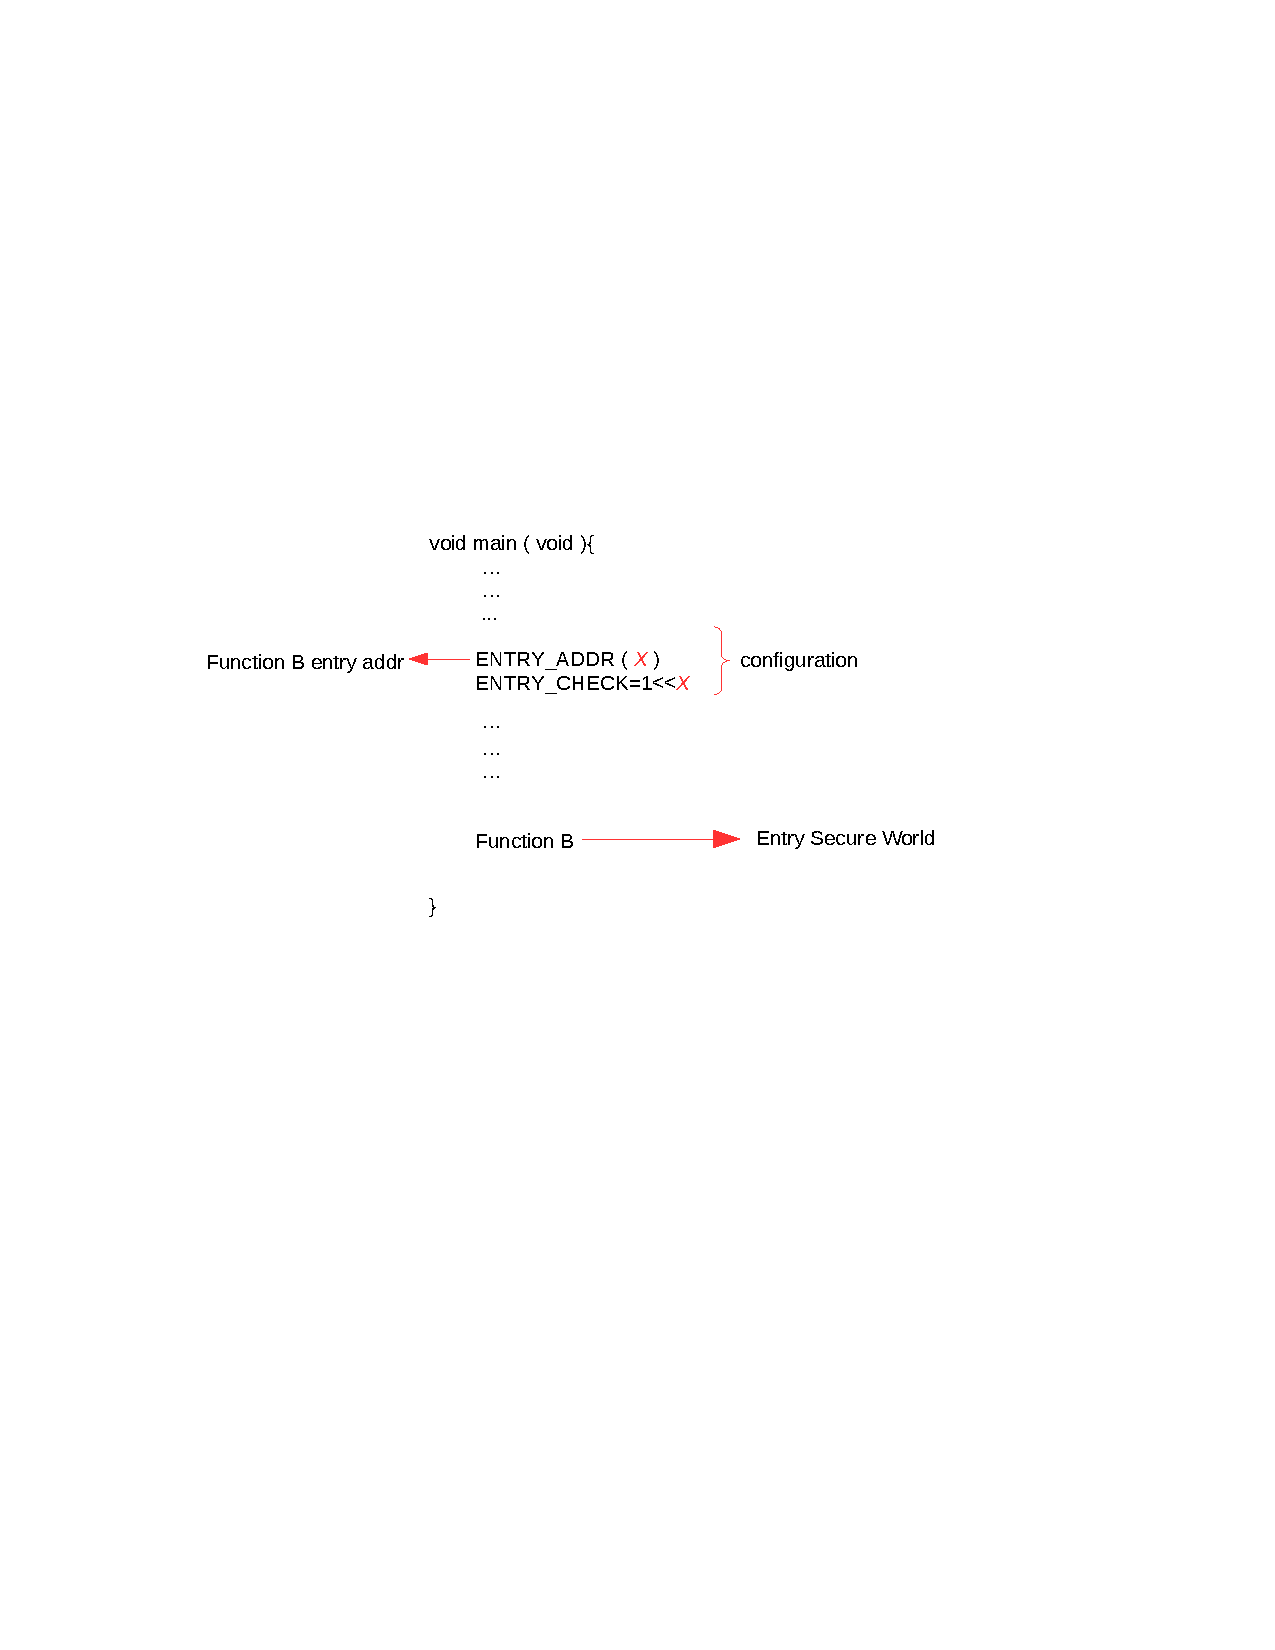
\includegraphics[width=0.7\textwidth]{./34-WCTRL/figures/world1toworld0.pdf}
    \caption{非安全世界切换到安全世界}
    \label{fig:34-WCTRL-nosafe-safe-switch}
\end{figure}

当 CPU 结束非安全世界应用程序，准备切换执行安全世界程序时：需要通过触发\textbf{中断}和\textbf{异常}的方式。经过配置后，当 World 控制器检测到触发的中断或异常后（即监测 CPU 是否执行到中断和异常入口），会自动切换到安全世界中。

\subparagraph{配置 World 控制器}

World 控制器的具体配置过程如下：

\begin{enumerate}
    \item 配置中断或异常的入口基地址 \hyperref[regdesc:WCLCORE0MTVECBASEREG]{WCL\_CORE\_0\_MTVEC\_BASE\_REG}。之后，World 控制器会按照以下规则，自动生成每个入口的监测地址。
    \begin{itemize}
    \item 异常的入口：\hyperref[regdesc:WCLCORE0MTVECBASEREG]{WCL\_CORE\_0\_MTVEC\_BASE\_REG} + 0x00
    \item 中断的入口：\hyperref[regdesc:WCLCORE0MTVECBASEREG]{WCL\_CORE\_0\_MTVEC\_BASE\_REG} + 4* \regindex{i} (\regindex{i} = 1\verb+~+31)
    \end{itemize}
    注意，该寄存器需与 CPU 的 \hyperref[regdesc:MTVEC]{mtvec} CSR 保持一致。当修改 \hyperref[regdesc:MTVEC]{mtvec} CSR 时，需要同步更新该寄存器。有关 \hyperref[regdesc:MTVEC]{mtvec} CSR 的更多信息，请见章节 \ref{mod:riscvcpu} \textit{\nameref{mod:riscvcpu}}。
    \item 配置 \hyperref[regdesc:WCLCORE0ENTRYCHECKREG]{WCL\_CORE\_0\_ENTRY\_CHECK\_REG} 使能对任意入口地址的监测（0 为禁用监测，1 为开始监测），可配置为同时监测多个入口。其中
    \begin{itemize}
        \item 比特 0 控制异常入口地址
        \item 比特 1\verb+~+31 控制对应 \regindex{x} 号中断入口地址 (\regindex{x} = 1\verb+~+31)
    \end{itemize}
    注意，本寄存器一次使能，长期有效。之后每次监测到入口地址的取指行为都会自动切换到安全世界，直至被禁用。
    此后，一旦 CPU 执行到以上监测的入口地址处即立刻将 CPU 切换到安全世界。
    \item 使能 \hyperref[regdesc:WCLCORE0MSTATUSMIEREG]{WCL\_CORE\_0\_MSTATUS\_MIE\_REG}， 寄存器开启世界切换记录表记录功能。否则，发生世界切换时，世界切换记录表不会更新。关于世界切换记录表详见 \ref{subsub:world_switch_table}。
\end{enumerate}

























\section{世界切换记录表} \label{subsub:world_switch_table}

通常情况下，CPU 会频繁进行世界切换且存在中断嵌套。为了能够回溯到切换至安全世界之前的世界属性，World 控制器还会记录世界切换日志，并将其保存在一系列寄存器中，即“世界切换记录表”。

\subsection{世界切换记录表寄存器的组成}

世界切换记录表由 32 个 \hyperref[regdesc:WCLCORE0STATUSTABLE0REG]{WCL\_CORE\_0\_STATUSTABLE\regindex{n}\_REG (\regindex{n}: 0-31)} 寄存器组成（结构如图 \ref{fig:wcl-world-status} 所示），其中 \hyperref[regdesc:WCLCORE0STATUSTABLE0REG]{WCL\_CORE\_0\_STATUSTABLE\regindex{x}\_REG} 寄存器记录 \regindex{x} 号入口的世界切换情况。

\begin{figure}[H]
    \centering
    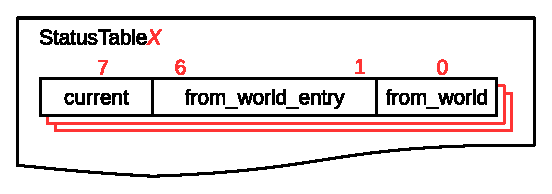
\includegraphics[width=0.5\textwidth]{./34-WCTRL/figures/statustable.eps}
    \caption{世界切换记录表}
    \label{fig:wcl-world-status}
\end{figure}
具体描述如下：
\begin{itemize}
    \item \hyperref[fielddesc:WCLCORE0FROMWORLD0]{WCL\_CORE\_0\_FROM\_WORLD\_\regindex{n}}：记录世界切换之前的世界信息。
    \begin{itemize}
        \item 0：安全世界
        \item 1：非安全世界
    \end{itemize}
    \item \hyperref[fielddesc:WCLCORE0FROMENTRY0]{WCL\_CORE\_0\_FROM\_ENTRY\_\regindex{n}}：记录发生跳转的入口，共 6 位。
    \begin{itemize}
        \item 0\verb+~+31:  表示当前是从另一个中断/异常程序跳转过来，其入口号为 0\verb+~+31 。
        \item 32: 表示切换之前不处于任何入口监测的中断。
    \end{itemize}
    \item \hyperref[fielddesc:WCLCORE0CURRENT0]{WCL\_CORE\_0\_CURRENT\_\regindex{n}}：表示该入口当前是否处于监测的中断中。当某个入口 \regindex{x} 发生中断时，
    \begin{itemize}
        \item 该入口对应的 \hyperref[fielddesc:WCLCORE0CURRENT0]{WCL\_CORE\_0\_CURRENT\_\regindex{x}} 域均将被更新为 1；
        \item 其余入口的 current 域均将更新为 0。
    \end{itemize}
\end{itemize}

\subsection{世界切换记录表寄存器的更新}\label{sec:wctrl-update-statetable}

假设初始状态下，CPU 处于非安全世界，所有 \hyperref[regdesc:WCLCORE0STATUSTABLE0REG]{WCL\_CORE\_0\_STATUSTABLE\regindex{n}\_REG(\regindex{n}: 0-31)} 寄存器为 0。接着，入口 9、入口 1 和入口 4 依次发生优先级更高的中断。

此时，世界切换记录表更新过程如下：
\begin{enumerate}
    \item 首先，9 号入口监测到中断发生。CPU 开始执行 9 号中断的入口地址时，世界切换记录表更新如图 \ref{fig:wcl-world-change0} 所示：
    \begin{figure}[H]
    \centering
    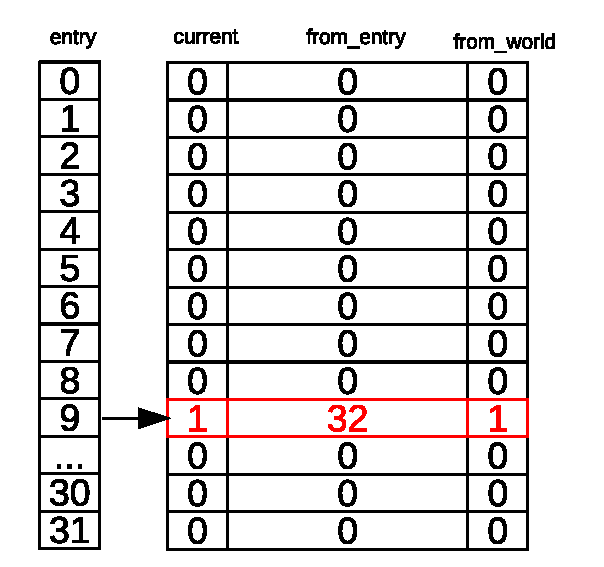
\includegraphics[width=0.3\textwidth]{./34-WCTRL/figures/world_table0.eps}
    \caption{中断嵌套流程示意图 - 9 号入口}
    \label{fig:wcl-world-change0}
    \end{figure}
    其中，\begin{itemize}
        \item \hyperref[regdesc:WCLCORE0STATUSTABLE0REG]{WCL\_CORE\_0\_STATUSTABLE9\_REG}
        \begin{itemize}
            \item \hyperref[fielddesc:WCLCORE0FROMWORLD0]{WCL\_CORE\_0\_FROM\_WORLD\_9} 域为 1，表示 CPU 在切换之前处于非安全世界。
            \item \hyperref[fielddesc:WCLCORE0FROMENTRY0]{WCL\_CORE\_0\_FROM\_ENTRY\_9} 域为 32，表示切换之前不处于任何入口监测的中断。
            \item \hyperref[fielddesc:WCLCORE0CURRENT0]{WCL\_CORE\_0\_CURRENT\_9} 域为 1，表示此时 CPU 正在 9 号入口监测的中断中。
        \end{itemize}
        \item 其他 \hyperref[regdesc:WCLCORE0STATUSTABLE0REG]{WCL\_CORE\_0\_STATUSTABLE\regindex{n}\_REG} 寄存器均保持不变。
    \end{itemize}
    \item 接着，1 号入口监测到一个更高优先级的中断。CPU 开始执行 1 号中断的入口地址时，世界切换记录表再次发生更新，如图 \ref{fig:wcl-world-change1} 所示：
        \begin{figure}[H]
        \centering
        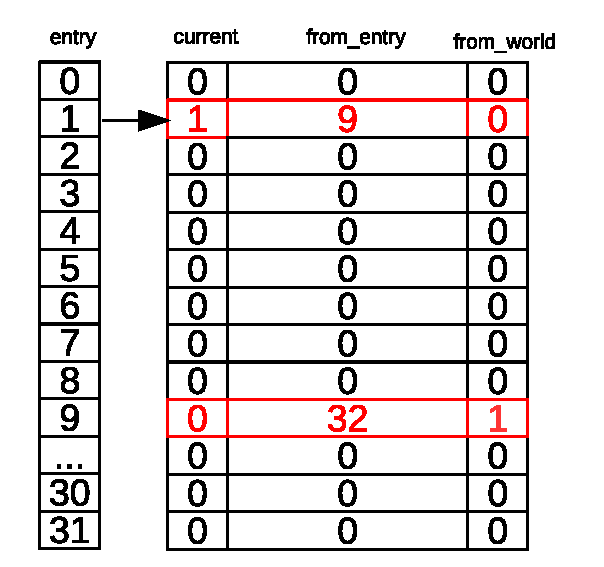
\includegraphics[width=0.3\textwidth]{./34-WCTRL/figures/world_table1.eps}
        \caption{中断嵌套流程示意图 - 1 号入口 }
        \label{fig:wcl-world-change1}
        \end{figure}
    其中，
    \begin{itemize}
        \item \hyperref[regdesc:WCLCORE0STATUSTABLE0REG]{WCL\_CORE\_0\_STATUSTABLE1\_REG}
        \begin{itemize}
            \item \hyperref[fielddesc:WCLCORE0FROMWORLD0]{WCL\_CORE\_0\_FROM\_WORLD\_1} 域为 0，表示 CPU 在切换之前处于安全世界。
            \item \hyperref[fielddesc:WCLCORE0FROMENTRY0]{WCL\_CORE\_0\_FROM\_ENTRY\_1} 域为 9，表示切换之前处于 9 号入口监测的中断。
            \item \hyperref[fielddesc:WCLCORE0CURRENT0]{WCL\_CORE\_0\_CURRENT\_1} 域更新为 1，表示此时 CPU 正在 1 号入口监测的中断中。
        \end{itemize}
        \item \hyperref[regdesc:WCLCORE0STATUSTABLE0REG]{WCL\_CORE\_0\_STATUSTABLE9\_REG}
        \begin{itemize}
            \item \hyperref[fielddesc:WCLCORE0CURRENT0]{WCL\_CORE\_0\_CURRENT\_9} 域更新为 0，表示此时 CPU 已经不在 9 号入口监测的中断中（进入 1 号入口中断的监控中）。
            \item \hyperref[fielddesc:WCLCORE0FROMWORLD0]{WCL\_CORE\_0\_FROM\_WORLD\_9} 域和 \hyperref[fielddesc:WCLCORE0FROMENTRY0]{WCL\_CORE\_0\_FROM\_ENTRY\_9} 域保持不变。
        \end{itemize}
        \item 其他 \hyperref[regdesc:WCLCORE0STATUSTABLE0REG]{WCL\_CORE\_0\_STATUSTABLE\regindex{n}\_REG} 寄存器均保持不变。
    \end{itemize}
        \item 接着，4 号入口又监测到一个更高优先级的中断。CPU 开始执行 4 号中断的入口地址时，世界切换记录表再次发生更新，如图 \ref{fig:wcl-world-change2} 所示：
        \begin{figure}[H]
            \centering
            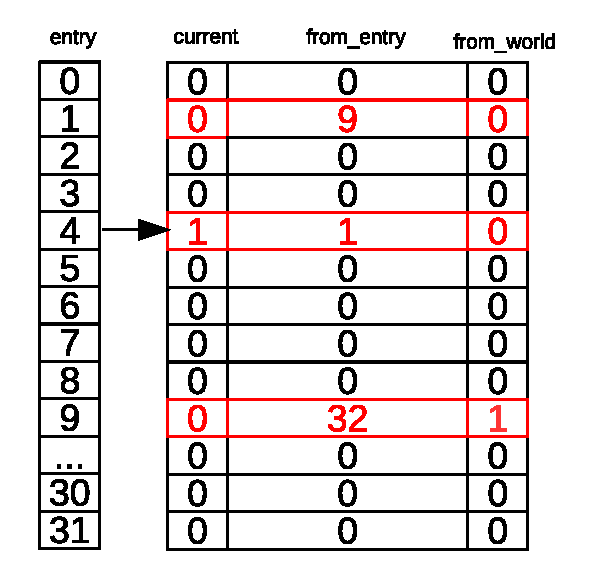
\includegraphics[width=0.3\textwidth]{./34-WCTRL/figures/world_table2.eps}
            \caption{中断嵌套流程示意图 - 4 号入口}
            \label{fig:wcl-world-change2}
        \end{figure}
        其中，
        \begin{itemize}
        \item \hyperref[regdesc:WCLCORE0STATUSTABLE0REG]{WCL\_CORE\_0\_STATUSTABLE4\_REG}
        \begin{itemize}
            \item \hyperref[fielddesc:WCLCORE0FROMWORLD0]{WCL\_CORE\_0\_FROM\_WORLD\_4} 域为 0，表示 CPU 在切换之前处于安全世界。
            \item \hyperref[fielddesc:WCLCORE0FROMENTRY0]{WCL\_CORE\_0\_FROM\_ENTRY\_4} 域为 1，表示切换之前处于 1 号入口监测的中断。
            \item \hyperref[fielddesc:WCLCORE0CURRENT0]{WCL\_CORE\_0\_CURRENT\_4} 域更新为 1，表示此时 CPU 正在 4 号入口监测的中断中。
        \end{itemize}
        \item \hyperref[regdesc:WCLCORE0STATUSTABLE0REG]{WCL\_CORE\_0\_STATUSTABLE1\_REG}
        \begin{itemize}
            \item \hyperref[fielddesc:WCLCORE0CURRENT0]{WCL\_CORE\_0\_CURRENT\_1} 域更新为 0，表示此时 CPU 已经不在 1 号入口监测的中断中（进入 4 号入口中断的监控中）。
            \item \hyperref[fielddesc:WCLCORE0FROMWORLD0]{WCL\_CORE\_0\_FROM\_WORLD\_1} 域和 \hyperref[fielddesc:WCLCORE0FROMENTRY0]{WCL\_CORE\_0\_FROM\_ENTRY\_1} 域保持不变。
        \end{itemize}
        \item 其他 \hyperref[regdesc:WCLCORE0STATUSTABLE0REG]{WCL\_CORE\_0\_STATUSTABLE\regindex{n}\_REG} 寄存器均保持不变。
\end{itemize}
\end{enumerate}

\subsection{世界切换记录表寄存器的读取} \label{sec:wctrl-read-table}

通过查看世界切换记录表，我们也可以了解世界切换前的世界以及是否发生中断嵌套等信息，从而能够正确恢复到世界切换前的状态。

具体方式如下（以图 \ref{fig:wcl-world-change2} 为例）：
\begin{enumerate}
    \item 查询 \hyperref[regdesc:WCLCORE0STATUSTABLECURRENTREG]{WCL\_CORE\_0\_STATUSTABLE\_CURRENT\_REG} 寄存器，得知目前 CPU 正处于 4 号入口监测的中断中。
    \item 查询 \hyperref[fielddesc:WCLCORE0FROMENTRY0]{WCL\_CORE\_0\_FROM\_ENTRY\_4} 域为 1，得知之前存在 1 号入口监测的中断。
    \item 查询 \hyperref[fielddesc:WCLCORE0FROMENTRY0]{WCL\_CORE\_0\_FROM\_ENTRY\_1} 域为 9，得知之前存在 9 号入口监测的中断。
    \item 查询 \hyperref[fielddesc:WCLCORE0FROMENTRY0]{WCL\_CORE\_0\_FROM\_ENTRY\_9} 域为 32，得知之前已经不存在其他入口监测的中断；此时，接着查询 \hyperref[fielddesc:WCLCORE0FROMWORLD0]{WCL\_CORE\_0\_FROM\_WORLD\_9} 域为 1，得知世界切换前处于非安全世界。
\end{enumerate}


\subsection{中断嵌套}

为支持中断嵌套，World 控制器提供了额外的配置来更新\nameref{subsub:world_switch_table}, 具体配置请参考下方章节\nameref{sec:wctrl-prog-step}。





\subsubsection{编程指南} \label{sec:wctrl-prog-step}

\textbf{处理 \regindex{A} 处的中断：\label{step:wctrl-start-interrput}}
    \begin{enumerate}
        \item 保存上下文。
        \item 使能 \hyperref[regdesc:WCLCORE0MSTATUSMIEREG]{WCL\_CORE\_0\_MSTATUS\_MIE\_REG} 寄存器，使能更新\nameref{subsub:world_switch_table}。
        \begin{itemize}
            \item RISC-V CPU 进入中断和异常 vector 后会自动关闭全局中断使能以避免中断嵌套，在保存完上下文之后软件可再次开启全局中断使能去响应更高级中断。
            \item World 控制器  \hyperref[regdesc:WCLCORE0MSTATUSMIEREG]{WCL\_CORE\_0\_MSTATUS\_MIE\_REG} 寄存器也支持全局中断使能类似的特性。当检测到任一入口触发后 \hyperref[regdesc:WCLCORE0MSTATUSMIEREG]{WCL\_CORE\_0\_MSTATUS\_MIE\_REG} 会自动清 0，需要软件在中断/异常服务程序里再次使能。注意，该寄存器应在打开全局中断使能之前进行配置。
        \end{itemize}
        \item 打开全局中断使能
        \item 正常执行中断服务程序。\label{step:interrupt-process-normal}
        \item 禁止全局中断使能。
        \item 查询 \regindex{A} 号入口的世界切换记录寄存器中的 \hyperref[fielddesc:WCLCORE0FROMENTRY0]{WCL\_CORE\_0\_FROM\_ENTRY\_\regindex{A}}：\label{step:interrupt_process_update}
            \begin{itemize}
                \item 32：表示所有中断均已处理，CPU 将返回正常程序。此时：
                \begin{enumerate}
                    \item 更新入口 \regindex{A} 的世界切换寄存器：更新  \hyperref[fielddesc:WCLCORE0CURRENT0]{WCL\_CORE\_0\_CURRENT\_\regindex{A}} 为 0，表示中断已不再 \regindex{A} 处。
                    \item 跳转至第 \ref{step:last-step} 步。
                \end{enumerate}
                \item 0-31：表示仍有未处理的中断，CPU 将跳转至入口 \regindex{B} 处的中断。此时：
                    \begin{itemize}
                        \item 更新入口 \regindex{A} 的世界切换寄存器：
                        \begin{itemize}
                            \item \hyperref[fielddesc:WCLCORE0CURRENT0]{WCL\_CORE\_0\_CURRENT\_\regindex{A}} 为 0，表示中断已不再 \regindex{A} 处。
                            \item \hyperref[fielddesc:WCLCORE0FROMWORLD0]{WCL\_CORE\_0\_FROM\_WORLD\_\regindex{A}} 和 \hyperref[fielddesc:WCLCORE0FROMENTRY0]{WCL\_CORE\_0\_FROM\_ENTRY\_\regindex{A}} 保持不变。
                        \end{itemize}
                        \item 更新入口 \regindex{B} 的世界切换寄存器：
                        \begin{itemize}
                            \item 更新 \regindex{B} 的  \hyperref[fielddesc:WCLCORE0CURRENT0]{WCL\_CORE\_0\_CURRENT\_\regindex{B}} 为 1，表示 CPU 将返回入口 \regindex{B}。
                        \end{itemize}
                    \end{itemize}
            \end{itemize}
        \item 准备退出中断。\label{step:last-step}
            \begin{enumerate}
                \item 查询需前往的世界：
                    \begin{itemize}
                        \item 如仍返回到安全世界，则跳转到第 \ref{step:final} 步。
                        \item 如需前往非安全世界，则切换至需要的世界，参考章节 \ref{sec:34-WCTRL-recommended-operation}。然后跳转到第 \ref{step:final} 步。
                    \end{itemize}
            \end{enumerate}
        \item 恢复中断使能, 恢复上下文并退出中断。 \label{step:final}
\end{enumerate}


\begin{tiplisting}
上述处理过程中的 \ref{step:interrupt_process_update} 和 \ref{step:last-step} 不能被高级中断打断，因此在执行这两个步骤之前应该将所有的中断关闭，处理完之后再将所有的中断打开。
\end{tiplisting}









\clearpage
\section{寄存器列表}\hypertarget{wctrl-reg-summ}{}

本小节的所有地址均为相对于 World 控制器基地址的地址偏移量（相对地址），具体基地址请见章节 \ref{mod:sysmem} \textit{\nameref{mod:sysmem}} 中的表 \ref{tab:sysmem-base-address}。

请查看章节 \hyperref[glossary-access-types]{\textit{寄存器的访问类型}}，了解“访问”列缩写的含义。

\subfile{\modulefiles/34-WCTRL-reg-summ__CN}


\clearpage
\section{寄存器}

本小节的所有地址均为相对于World 控制器基地址的地址偏移量（相对地址），具体基地址请见章节 \ref{mod:sysmem} \textit{\nameref{mod:sysmem}} 中的表 \ref{tab:sysmem-base-address}。



\subfile{\modulefiles/34-WCTRL-reg__CN}

\end{document}
